%                                                                 aa.dem
% AA vers. 8.2, LaTeX class for Astronomy & Astrophysics
% demonstration file
%                                                       (c) EDP Sciences
%-----------------------------------------------------------------------
%
%\documentclass[referee]{aa} % for a referee version
%\documentclass[onecolumn]{aa} % for a paper on 1 column  
%\documentclass[longauth]{aa} % for the long lists of affiliations 
%\documentclass[rnote]{aa} % for the research notes
%\documentclass[letter]{aa} % for the letters 
%\documentclass[bibyear]{aa} % if the references are not structured 
% according to the author-year natbib style

%
\documentclass{aa}  

%
\usepackage{graphicx}
%%%%%%%%%%%%%%%%%%%%%%%%%%%%%%%%%%%%%%%%
\usepackage{txfonts}
%%%%%%%%%%%%%%%%%%%%%%%%%%%%%%%%%%%%%%%%
%\usepackage[options]{hyperref}
% To add links in your PDF file, use the package "hyperref"
% with options according to your LaTeX or PDFLaTeX drivers.
%
\begin{document} 


   \title{Simulations of the Dynamics Generated by Solar Global}

   \subtitle{ Oscillating Eigenmodes Generated in the Solar Atmosphere}


   \author{M.K.Griffiths,
          \inst{1}\fnmsep\thanks{Just to show the usage
          of the elements in the author field}
          V.Fedun\inst{2}
          \and
         R.Erd\'{e}lyi\inst{3}
          }

   \institute{Corporate Information and Computing Services, The University of Sheffield, 10-12 Brunswick Street, Sheffield, S10 2FN, UK\\
              \email{m.griffiths@sheffield.ac.uk}
           \and
                Department of Automatic Control and Systems Engineering, The University of Sheffield, Mappin Street, Sheffield, S1 3JD, UK\\
              \email{v.fedun@sheffield.ac.uk}
         \and
            Solar Physics and Space Plasma Research Centre ($SP^{2}RC$), School of Mathematics and Statistics, University of Sheffield, Hicks Building, Hounsfield Road, S7 3RH, UK\\
             \email{robertus@sheffield.ac.uk}
             \thanks{The university of heaven temporarily does not
                     accept e-mails}
             }



   \date{Received September 15, 1996; accepted March 16, 1997}

% \abstract{}{}{}{}{} 
% 5 {} token are mandatory
 
  \abstract
  % context heading (optional)
  % {} leave it empty if necessary  
   { The solar atmosphere exhibits a diverse range of wave phenomena one of the earliest to be discovered was the five minute oscillation, the p-mode. The solar p modes are generated by global resonant oscillations and turbulent motions just beneath the photosphere. The resulting propagation of this wave energy into the solar atmosphere may be used as a diagnostic tool to predict some of the physical characteristics of the  suns atmospheric layers.Report a study of synthetic photospheric oscillations in both non magentic and magnetic  model of the quiet sun}
  % aims heading (mandatory)
   {To investigate the dynamics in the solar atmosphere which are generated by solar global eigenmodes of oscillation and to understand mechanisms of leakage of 5 min global oscillations into the atmosphere. Understand the conditions under which chromospheric dynamics evolve as a result of the 5 minute global oscillations - (spicules, waves)
}
  % methods heading (mandatory)
   {  We report on a series of hydrodynamicsl simulations modelling a realistic solar atmosphere using a driver located at 0.5Mm above the temperature minimum. With the objective of recreating atmospheric motions generated by global resonant oscillation the driver is spatially structured and is extended in a sinusoidal profile arcoss the base of the computational model.  To carry out the simulations, we employed our the MHD code SMAUG (Sheffield MHD Accelerated Using GPUs). A combination of the VALIIIC and McWhirter solar atmospheres and coronal density profiles were used as the background equilibrium
model in the simulations. Vertical and horizontal harmonic sources, located at the footpoint region of the open magnetic flux tube, are incorporated in the calculations, to excite oscillations in the domain of interest.}
  % conclusions heading (optional), leave it empty if necessary 
   {Our results demonstrate the conversion of modes with a period of 30s to a mode with a period of 180s, demonstrating that the Chromosphere is a source of 180s modes. The results inidicate a shift in frequency arising from interference between the driven waves and reflections from the transition layer.}

   \keywords{magnetohydrodynamics (MHD) --
                oscillations --
                MHD waves --
                solar atmosphere
               }

   \maketitle
%
%________________________________________________________________

\section{Introduction}

The solar atmosphere exhibits a diverse range of wave phenomena. The first Observations of \cite{Leighton1960}  reported vertical motions on the solar surface with an amplitude of 300-400m/s with a period of 296s observations of Ca K band. These ubiquitous oscillations are referred to as the p-modes
The idea that these motions result from standing acoustic waves in the solar interior was proposed by Ulrich 1970  \cite{Ulrich1970} Reported that vertical wavelength comparable to horizontal wavelength and is roughly 1000-5000km.    \cite{Leibacher1971}.  These modes are pressure waves, the main restoring force for these oscillations is the pressure the 5 minute oscillation is the main manifestation of these modes. solar photosphere constant buffeting and movement driven by periodic and random motions e.g turbulent motions in photosphere or global effects such as those induced by p modes. The solar p modes are generated by global resonant oscillations and turbulent motions just beneath the photosphere.  These resonant modes are reflected at the surface by the steep change in density. The increase of the sound speed causes refraction.   The resulting propagation of this wave energy into the solar atmosphere may be used as a diagnostic tool to predict  physical characteristics of the  suns atmospheric layers. We report on a series of hydrodynamical simulations modelling a realistic solar atmosphere using a driver located at 0.5Mm above the temperature minimum. The objective of recreating atmospheric motions generated by global resonant oscillation the driver is extended in a sinusoidal profile arcoss the base of the computational model. The work presented here considers both hydrodynamic and magnetohydrodynamic scenarios. There is a significant body of work reporting on observational, theoretical and computational studies of p-mode phenomena. We briefly summarise some of this work here a detailed review was prepared by \cite{Khomenko2013}. The upward propagating acoustic shocks in the solar chromosphere was reported by Carlson Stein 1992  \cite{Carlsson1992}. The study used a 1D comutational model with a realistic model of the solar atmosphere and a model of radiative transfer. The resulting models of the generation of CaK2V bright points from acoustic waves with periods of 30, 180, and 300 s demonstrated that a 180s periodic driver produced results consistent with observations.

Considering the magnetohydrodynamic modes we compare our results to the study undertaken by  \cite{Hindman1996}, hre driven acoustic Oscillations within a vertical magnetic field  was considered. The study was extended by \cite{James2003} who demonstrated that the inclined magnetic field lines provide the favourable conditions for leakage of p-modes into solar atmosphere and generation of spicules. Marsh \cite{Marsh2006} provided evidence of signal propagation from the transition region to corona 3 min period band, such propagation occured along fieldlines this is also reported by \cite{Zhukov2002}. A recurring theme in many results is the observation that 3 min oscillations at transition region are related to 5 min global p-modes. There are two main view points for considering the mode conversion behaviour. These are to consider the chromosphere as resonant cavity and the behaviour of thecut off frequency.

A. Vecchio et al 2008  \cite{Cauzzi2008} use IBIS imaging data to 
identify the spatio-temporal occurrence of the acoustic shocks. We compare it with the photospheric dynamics by means of both Fourier and wavelet analysis, and study the influence of magnetic structures. portions of the internetwork regions undergo very few shocks, as "shadowed" by the horizontal component of the magnetic field. The latter is betrayed by the presence of chromospheric fibrils, observed in the core of the CaII line as slanted structures with distinct dynamical properties. The shadow mechanism appears to operate also on the very small scales of inter-network magnetic elements, and provides for a very pervasive influence of the magnetic field even in the quietest region analyzed. The observational results of Roth et al  \cite{Roth2010} provide evidence for the excitation of solar acoustic oscillations. The observed oscillations were excited by turbulent flows  in the intergranular lanes. The observations using the Imax instrument on the Sunrise observatory the turbulent downdrafts in the dark intergranular lanes are primary targets. So-called acoustic events, which are individual sunquakes with epicenters near the solar surface and located in the intergranular lanes, are assumed to feed continuously energy into the resonant p-modes of the Sun. Roth presents wavefronts rippling near a granule and oriented along the direction of the intergranular lane. It is understood that magnetic field lines suppress the p-mode oscillations \cite{Gascoyne2011} Sensitivity of p-mode absorption on magnetic region properties and kernel functions This has been corroborated further by the work of \cite{Jain2011} demonstrating that the Interaction of p modes with a collection of thin magnetic tubes (article) recently konkol et al (2012)  \cite{Konkol2012} have demonstrated that velocity pulses result in oscillatory phenomena with a periods of a few minutes. There two dimensional simulations demnstrate that the periods of the oscillations are dependent on the  amplitude and vertical location of the initial pulse. There model considers such propagation in a magnetised atmosphere with a non vertical field. Observations of the sausage pinch instability in the solar corona have been made with the SDO/AIA  \cite{Srivastava2013}


There is a large body of computational work already undertaken Among others the following \cite{Fedun 2009} et al study the Oscillatory Response of the 3D Solar Atmosphere to the Leakage of Photospheric Motion results are discussed in detail: i) High-frequency waves are shown to propagate from the lower atmosphere across the transition region, experiencing relatively low reflection, and transmitting most of their energy into the corona; ii) the thin transition region becomes a wave guide for horizontally propagating surface waves for a wide range of driver periods, and particularly at those periods that support chromospheric standing waves; iii) the magnetic field acts as a waveguide for both high- and low-frequency waves originating from the photosphere and propagating through the transition region into the solar corona.

Previous work has considered either point source drivers with a gaussian velocity distribution Other work e.g. by K. Murawski, T.V. Zaqarashvili (2010) \cite{Murawski2010} has demontrated that The numerical simulations show that the strong initial pulse may lead to the quasi periodic rising of chromospheric material into the lower corona in the form of spicules Khomenko and SantaMaria \cite{Khomenko2012}. The objective of the work presented here  is to characterise the dynamics generated by these solar global oscillating eigenmodes generated in the solar atmosphere.  These modes ARE some sort of global eigenmodes. The coherence length of eigenoscillations at the photoshphere is about a few Mm, and the power peaks at around 3-5 mins. We consider the behaviour of these modes in a non magnetic atmosphere, an atmosphere with a uniform magnetic field and with magnetic flux tubes of different widths.



%__________________________________________________________________



\section{Numerical Computation Methods and Excitation Drivers}
Before considering the implementation of the SMAUG application we now recall briefly the numerical solution method employed for the SAC code.  The 3D numerical simulations described here here were undertaken using SMAUG, the GPU implementation of the Sheffield Advanced Code \cite{Shelyag2008}. SMAUG is a numerical MHD solver that allows the simulation of the various physical processes in magnetised plasmas.  With the upper boundary of our model in the Solar Corona and the lower boundary in the photosphere the SAC code is well suited for modelling the leakage of wave energy from the photopshere, through the transition zone and into the photosphere. With open boundary conditions for the lower and upper boundaries it is possible to model wave propagation for time scales characterised by the 5 minute p-mode induced oscillations. The general system of MHD equations are
\begin{equation}\label{eqdens}
{{\partial \rho}\over{\partial t}}+\nabla\cdot\left( {\bf v}\rho\right)=0,
\end{equation}

\begin{equation}\label{eqmom}
{{\partial ( \rho {\bf v})}\over{\partial t}}+\nabla\cdot\left( {\bf v}\rho {\bf v}-{\bf B B}\right)+\nabla p_t=\rho{\bf g},
\end{equation}

\begin{equation}\label{eqe}
{{\partial e}\over{\partial t}}+\nabla.\left({\bf v}e-{\bf B B}\cdot{\bf v}+{\bf v}p_{t}\right)+\nabla p_t=\rho{\bf g}\cdot{\bf v},
\end{equation}

\begin{equation}\label{eqb}
{{\partial{\bf B}}\over{\partial t}} +\nabla \cdot\left(  {\bf vB}-{\bf Bv}\right)=0.
\end{equation}

In these equations $\rho$ is the mass density, $  \bf { v} $ is the velocity,   $ \bf B$ is the magnetic field, $\it{e}$ is the energy density, $p_{t}$ is the total pressure and $\bf g$ is the gravitatioanl acceleration vector.

The total pressure $p_{t}$ is written as
\begin{equation}\label{eqpt}
p_{t}=p_{k}+{{\bf B}^{2}\over{2}},
\end{equation}
where $p_k$ is the kinetic pressure given by
\begin{equation}\label{eqpk}
p_{k}=(\gamma - 1)( e-{{\rho \bf v }^{2}\over{2}}-  {{\bf B}^{2}\over{2}} ).
\end{equation}

The equations \eqref{eqdens} to \eqref{eqpk} are applicable to an ideal compressible plasma. The SAC code is based on perturbed versions of these equations, thus the variables $\rho $, $e$ and  $\bf B$ are expressed in terms of perturbed and background quantities as
\begin{equation}
\rho = \tilde{\rho}+\rho _{b},
\end{equation}
\begin{equation}
e = \tilde{e}+e _{b},
\end{equation}
\begin{equation}
\bf B = \tilde{\bf B}+{\bf B}_{\it{b}}.
\end{equation}
where $\tilde{\rho}$ is the  perturbed density,  $\tilde{e}$ is the perturbed energy and $\tilde{\bf B}$  is the perturbed magnetic field. The background quantities with a subscript $\it{b}$ do not change in time, as we assume a magneto-hydrostatic equilibrium of the background plasma which may have a gravitational field present, denoted by $\bf g$. Hyper-diffusion and hyper-resistivity \cite{Caunt2001}
are implemented to achieve numerical stability of the computed solution of the MHD equations.  The full set of MHD equations, including the hyper-diffusion source terms are shown in Appendix A.




\begin{equation}\label{eqpointdriver}
V_{z}=A \sin{\left({2\pi t}\over{T_s} \right)  }  \exp{\left( -{(x-x_0)^{2}}\over{\Delta x^{2}} \right) } \exp{\left( -{(z-z_0)^{2}}\over{\Delta z^{2}} \right) },
\end{equation}


\begin{equation}\label{eqsindriver}
V_{z}=A \sin{\left({2\pi t}\over{T_s} \right)  }\sin{\left(  {(n+1)\pi x}\over{L_x} \right)} \exp{\left( -{(z-z_0)^{2}}\over{\Delta z^{2}} \right) },
\end{equation}


\begin{equation}\label{eqsindriver3d}
V_{z}=A_{nm} \sin{\left({2\pi t}\over{T_s} \right)  }\sin{\left(  {(n+1)\pi x}\over{L_x} \right)}   \sin{\left(  {(m+1)\pi y}\over{L_y} \right)}    \exp{\left( -{(z-z_0)^{2}}\over{\Delta z^{2}} \right) },
\end{equation}


We undertaken simulations for different modes of oscillation where the mode is define by the index $\it{n}$ and $\it{m}$ in equation \eqref{eqsindriver3d} and \eqref{eqsindriver}. Since we are investigating the leakage of energy into the solar atmosphere it is necessary 

\begin{equation}\label{driverenergy}
E_{nm}(z,t)= \rho A_{nm} I_{nm}  \sin{\left({2\pi t}\over{T_s} \right)  }    \exp{\left( -{(z-z_0)^{2}}\over{\Delta z^{2}} \right) },
\end{equation}

\begin{equation}\label{driverenergyintegral}
I_{nm}=  \int_{-L/2}^{+L/2} \int_{-L/2}^{+L/2} \sin{\left({2\pi t}\over{T_s} \right)  }\sin{\left(  {(n+1)\pi x}\over{L_x} \right)}   \sin{\left(  {(m+1)\pi y}\over{L_y} \right)}   ,
\end{equation}

\begin{equation}\label{driveramplituderelatinl}
A_{nm}=\frac{2A_{00}}{(n^2+m^2+2(n+m)+2)}   ,
\end{equation}


%__________________________________________________________________


\section{Solar Atmospheric Model}
In order to model the behaviour of physical processes in the Solar atmosphere a physically representative model is needed. An option is the use of a parametrisation of the tempearture of the solar atmosphere which may be a smoothed step function profile  \cite{Murawski2010}. Results have demonstrated the need for observationally derived semi-emprical models of the solar atmosphere. There is much discussion about model validity and the work undertaken to demonstrate the reliability of the assumptions used to construct realistic models of the solar chromosphere \cite{Carlsson1995}, \cite{Kalkofen2012}. The contention arises from the dynamical nature of the solar chromosphere for example local dynamo action has been suggested as a mechanism of Joule heating in the solar chromosphere \cite{Leenaarts2011}. The model atmosphere employed here is an observationally derived semi-empirical representation of the quiet sun. With the fundamental assumption of hydrostatic equilibrium a model of the chromosphere in equilibrium is constructed using the VALIIc model \cite{Vernazza1981}. For the region of the solar atmosphere above 2.5Mm the results of the energy balance model of solar coronal heating has been used this model also includes an acoustic contribution comparable to the hydrostatic pressure \cite{McWhirter1975}

%FIGURE 1 here caption:Illustration highlighting the model configuration.\\

\begin{figure*}[h]
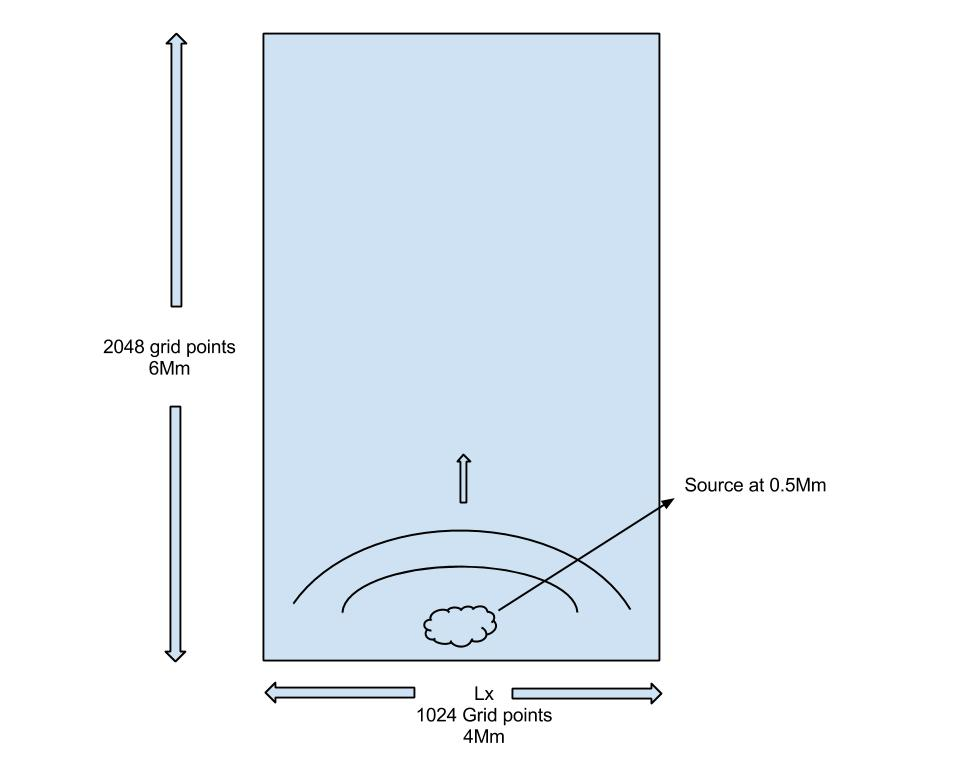
\includegraphics[scale=0.5]{images/solarmodel_fig1.jpg}
\caption{Illustration highlighting the model configuration. }
\end{figure*}


%FIGURE 2 here caption:Temperature and Density Profiles Used for the Model Atmosphere.\\

\begin{figure*}[h]
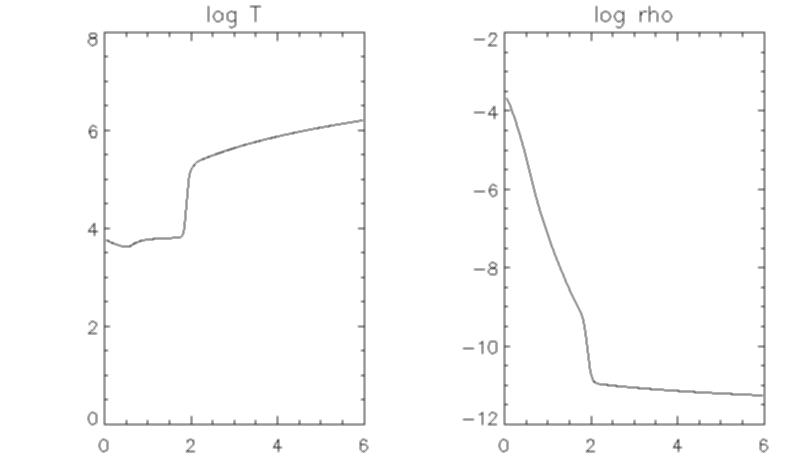
\includegraphics[scale=0.7]{images/VAL3C_fig2.jpg}
\caption{Temperature and Density Profiles Used for the Model Atmosphere. }
\end{figure*}

%FIGURE 3 here caption:Sound Speed Profile for the Model Atmosphere.\\

\begin{figure*}[h]
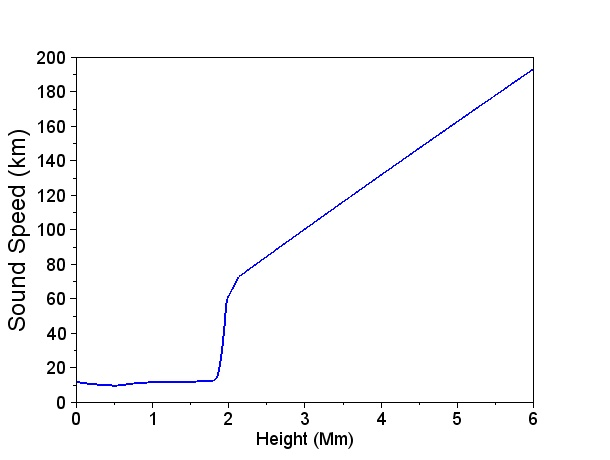
\includegraphics[scale=0.7]{images/soundspeedVAL3C_profile_fig3.jpeg}
\caption{Sound Speed Profile for the Model Atmosphere. }
\end{figure*}






%__________________________________________________________________


\section{Hydrodynamic Simulations}

In this section we present the result of the application of a vertical velocity driver located at the photosphere this acoustic p-mode driver excites waves which propagate into the atmosphere. We consider drivers with a time period of 30s, 180s and 300s. The synthetic driver with period 300s used in the simulations corresponds to the dominant five minute solar global p mode. Here we extend the  work of \cite{Malins2007A} by applying a complex spatially structured driver across the lower boundary of a realisitc 3D model of the Solar atmosphere and mimicing solar global oscillations. This driver may be represented as an ensemble of solar global eigenmodes.  In the real Sun photospheric p-mode oscillations have a horizontal wavelength and coherence, simulations were run for three typical cases of such horizontally coherent drivers. These are a driver with a wavelength of 8 Mm applied along the middle 4 Mm of the base of the computational domain with sinusoidal horizontal amplitude dependence (a “fundamental mode”) and a driver with wavelength 4 Mm applied the same way (the “first harmonic”) a second harmonic with wavelength 2Mm was also considered. \cite{Malins2007A} the work here considered times 2676s demonstrating structures evolving in the transition zone. The work presented in  \cite{Malins2007A} was applied to a 2 dimensional atmosphere. In addition to the consideration different blending of harmonics are model is 3D. The synthetic driver is given by \eqref{eqsindriver} it has a coherence length $L_{0}$ of $4Mm$, the width $\Delta z$  is $4km$ and the vertical location is the temperature minimum which is $0.5Mm$ above the lower boundary of the model i.e. the photosphere. The point driver described by \eqref{eqpointdriver} has width  $Delta x$ of $4Mm$, the width $\Delta z$  is $4km$$\Delta z$  is $4km$
Owing to the high gradients, partial reflection of acoustic waves at all frequencies is expected at the transition region. The transition region is the upper boundary of the chromospheric cavity, it has been previously suggested that this is the source of three-minute transition-region oscillations \cite{Leibacher1982}.

For the fundamental modes  illustrated in figure 4, 5 and 6 we observe that there is no significant structure at the transition zone. However, the 30s mode is particulalry interesting detailed movies demonstrate the rapid expansion of the plume as it crosses the transition zone this is accompanied with an increase in the transverse velocity this observationi is true for both 180s, 30s and 300s driver scenarios. As the mode order is increased from $n=0$, to $n=1$ and then $n=2$ its is observed that transition region structuring becomes apparent and is more reminiscent of the observations of \cite{Malins2007B}.




 



%FIGURE 4 here caption:Three-dimensional snapshots of the evolution of Vz showing the development of the initial perturbation in the nonmagnetic equilibrium generated 
%by the 30-second-period driver (in ms−1) at the times (a) t = 112 seconds, (b) t = 216 seconds, (c) t = 244 seconds, and (d) t = 316 seconds. 
%The z-axis corresponds to height measured in megameters and the x and y horizontal axes are parallel to the solar surface.\\

\begin{figure*}[h]\label{fig30svz_vt_mode0}
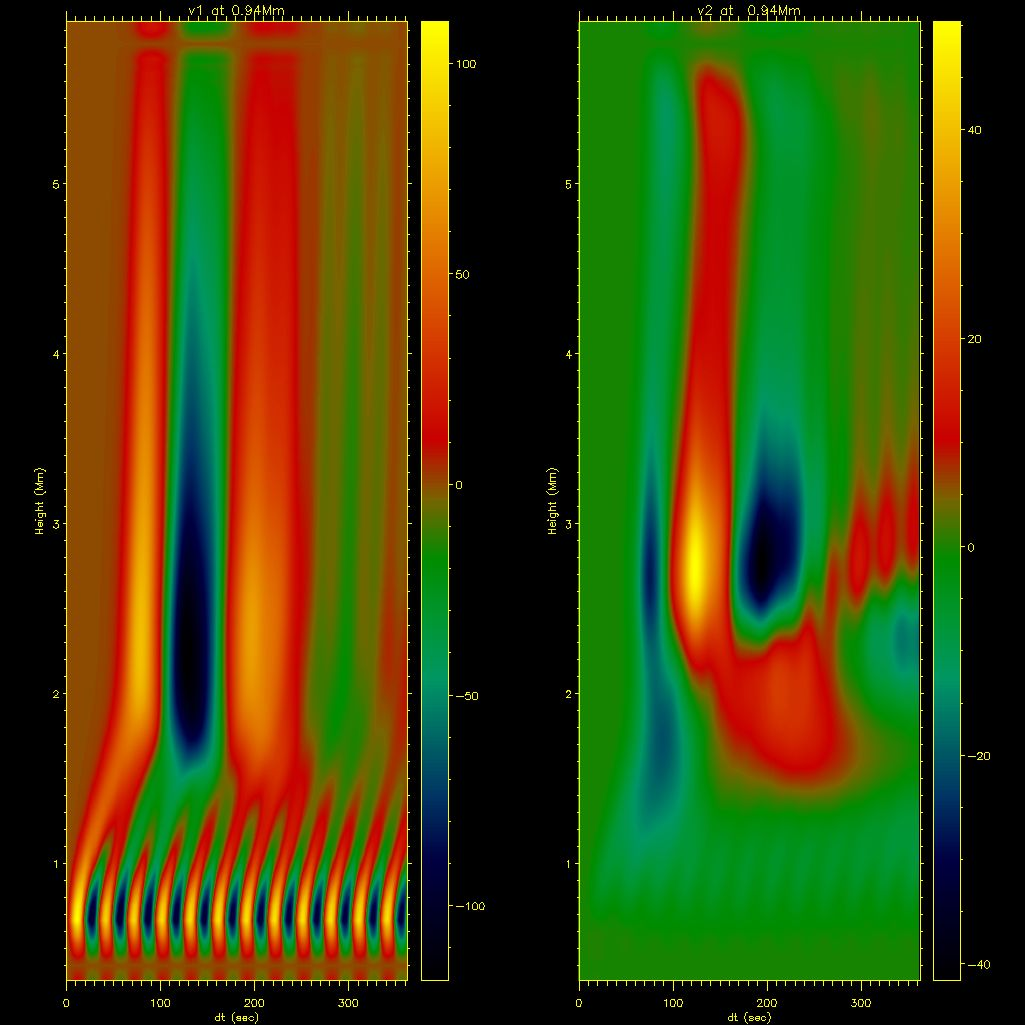
\includegraphics[scale=0.5]{images/pm30s_sindrv_n0_4b03d_dt.jpg}
\caption{Three-dimensional snapshots of the evolution of Vz showing the development of the initial perturbation in the nonmagnetic equilibrium generated by the 30-second-period driver (in ms−1) at the times (a) t = 112 seconds, (b) t = 216 seconds, (c) t = 244 seconds, and (d) t = 316 seconds. The z-axis corresponds to height measured in megameters and the x and y horizontal axes are parallel to the solar surface. }
\end{figure*}





%FIGURE 7 here caption:Distance time plot for fundamental model with 30s period for the z and y component of the velocity. The section  is taken at 0.94Mm across the box.\\

\begin{figure*}[h]\label{fig30dt_mode0}
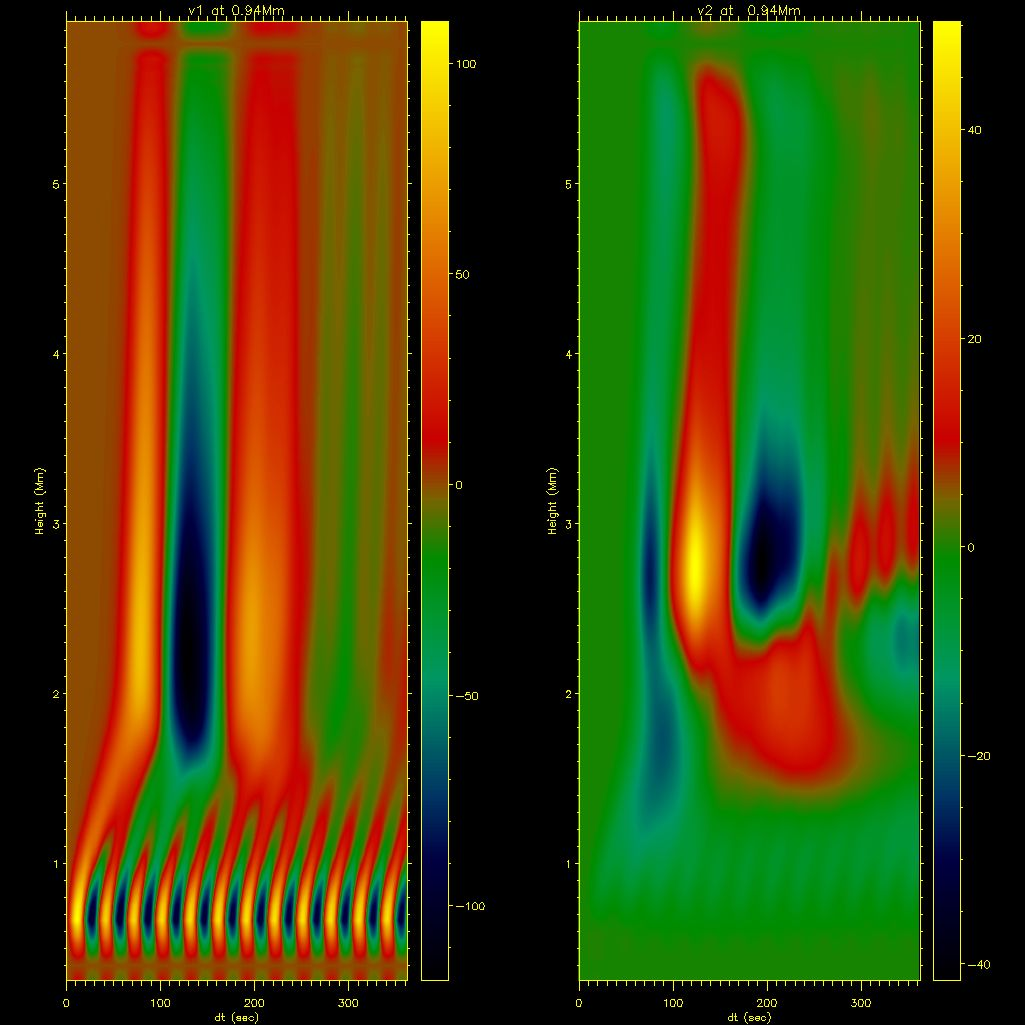
\includegraphics[scale=0.5]{images/pm30s_sindrv_n0_4b03d_dt.jpg}
\caption{Distance time plot for fundamental model with 30s period for the z and y component of the velocity. The section  is taken at 0.94Mm across the box. }
\end{figure*}



Figure \figref{fig30svz_vt_mode0} shows three-dimensional snapshots of the evolution of $V_{z}$. This is for the fundamental mode driver with a period of $30s$ for the case of a nonmagnetic configuration.The figure shows profiles obtained at the times (a) t = 112 seconds, (b) t = 216 seconds, (c) t = 244 seconds, and (d) t = 316 seconds. The distance-time plot in figure \figref{fig30dt_mode0} shows a plot of the z-component of the velocity at different altitudes through the atmosperic configuration and at different time steps. The plot shows clearly the conversion of the 30s chromospheric mode to a slower mode propagating with a period of 180s \cite{Leibacher1982}. 








%FIGURE 8 here caption:Distance time plot for fundamental model with 180s period for the z and y component of the velocity. The section  is taken at 0.94Mm across the box.\\

\begin{figure*}[h]
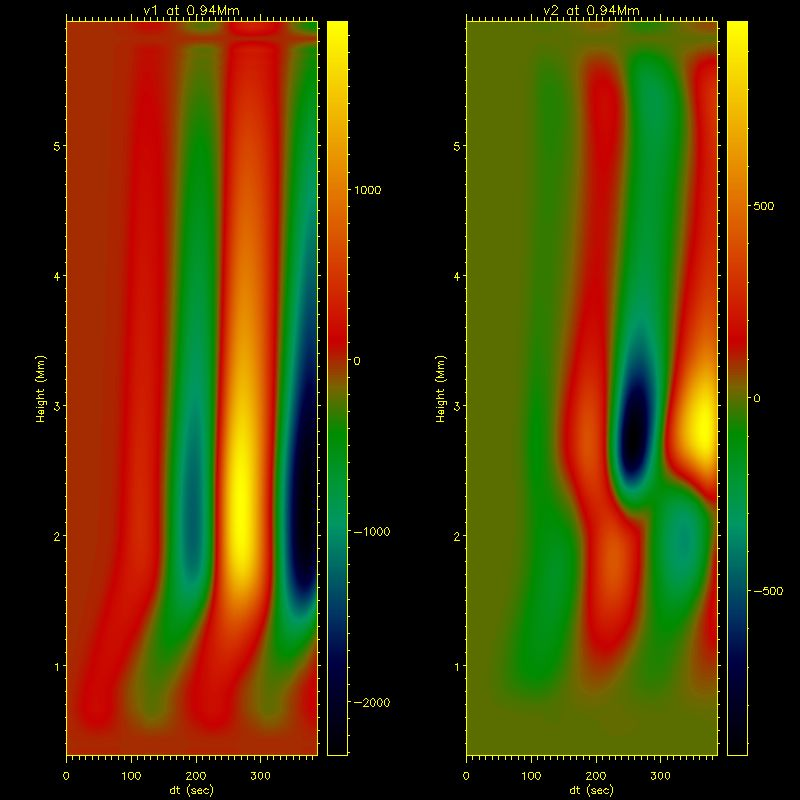
\includegraphics[scale=0.5]{images/pm180s_sindrv_n0_6b0_3d_h1dt.jpg}
\caption{Distance time plot for fundamental model with 180s period for the z and y component of the velocity. The section  is taken at 0.94Mm across the box. }
\end{figure*}


%FIGURE 9 here caption:Distance time plot for fundamental model with 300s period for the z and y component of the velocity. The section  is taken at 0.94Mm across the box. \\

\begin{figure*}[h]
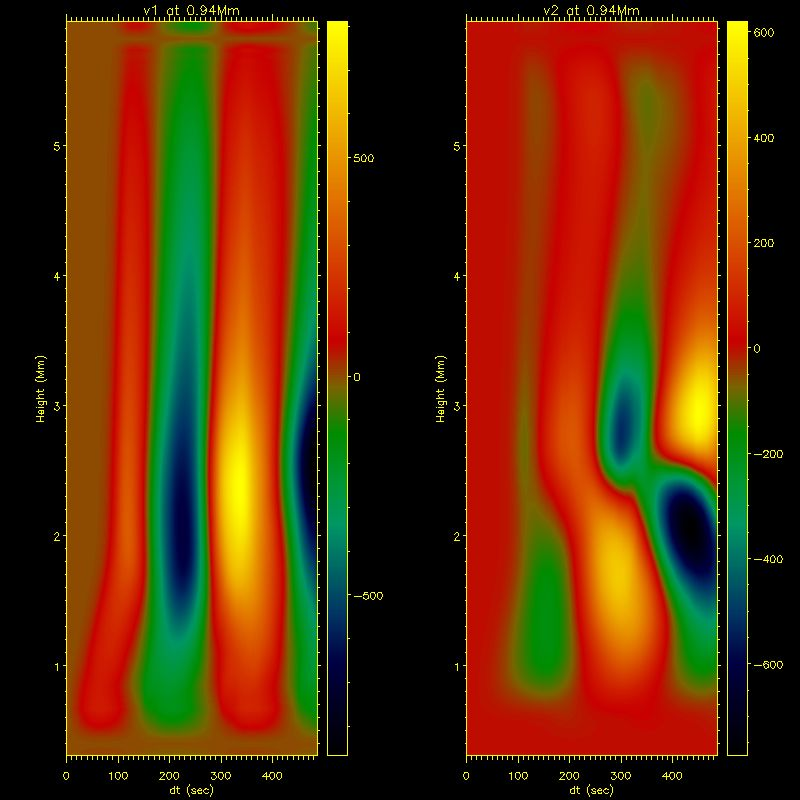
\includegraphics[scale=0.5]{images/pm300s_sindrv_n0_5b03d_h1dt.jpg}
\caption{Distance time plot for fundamental model with 300s period for the z and y component of the velocity. The section  is taken at 0.94Mm across the box. }
\end{figure*}














%FIGURE 10 here caption:A three dimensional snapshot showing the vertical component of the velocity for the 30s driver for $t=104s$, $t=119s$, $t=134s$ and $t=149s$ \\

\begin{figure*}[h]
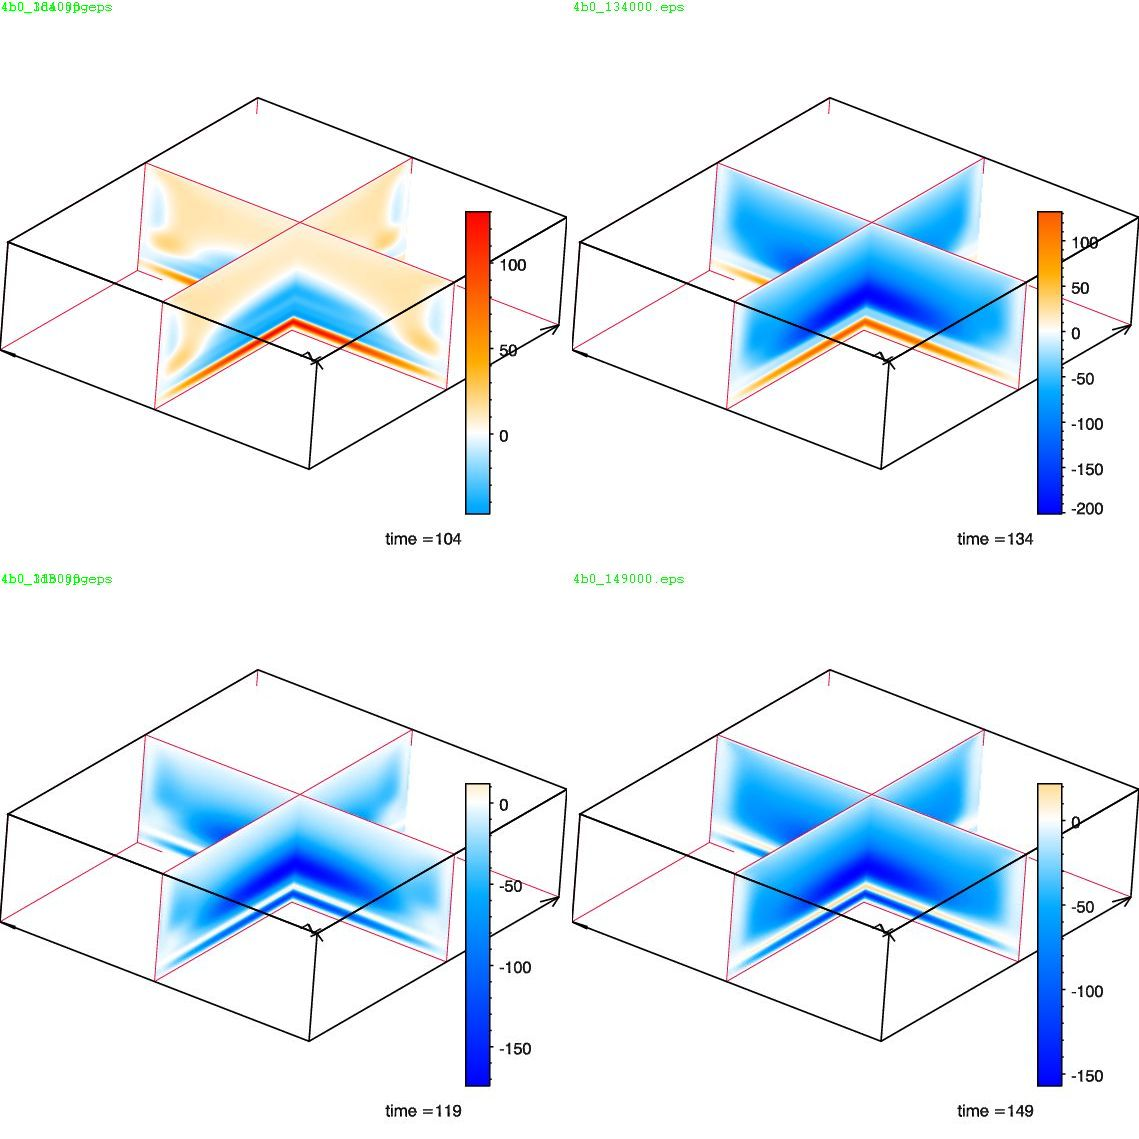
\includegraphics[scale=0.5]{images/4b0_3d.jpg}
\caption{A three dimensional snapshot showing the vertical component of the velocity for the 30s driver for $t=104s$, $t=119s$, $t=134s$ and $t=149s$. }
\end{figure*}


%FIGURE 11 here caption:A three dimensional snapshot showing the vertical component of the velocity for the 300s driver for $t=104s$, $t=119s$, $t=134s$ and $t=149s$ \\

\begin{figure*}[h]
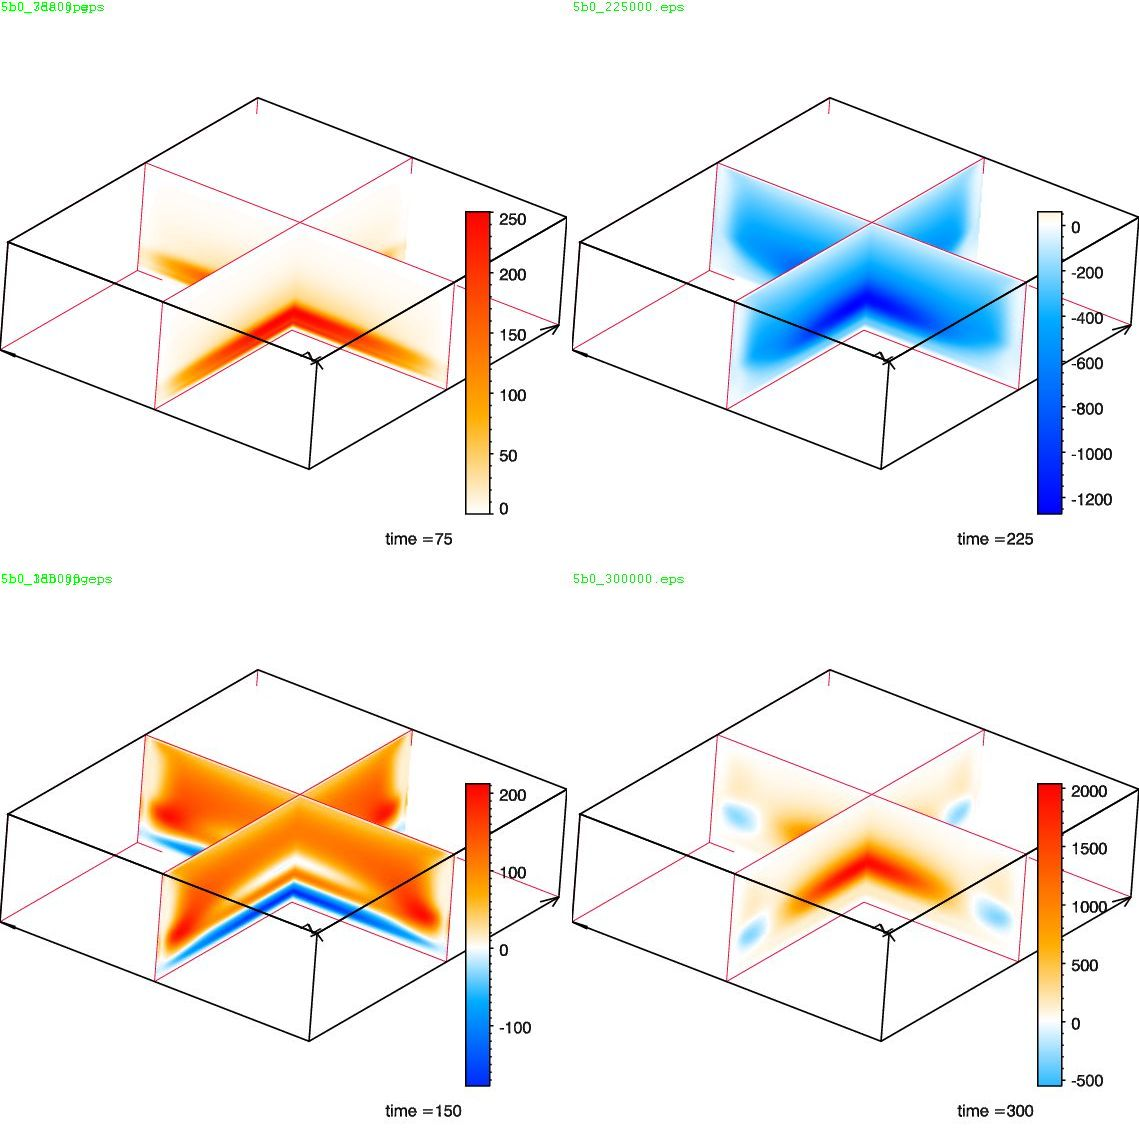
\includegraphics[scale=0.5]{images/5b0_3d.jpg}
\caption{A three dimensional snapshot showing the vertical component of the velocity for the 300s driver for $t=104s$, $t=119s$, $t=134s$ and $t=149s$. }
\end{figure*}


%FIGURE 12 here caption:A three dimensional snapshot showing the vertical component of the velocity for the 180s driver for $t=104s$, $t=119s$, $t=134s$ and $t=149s$\\

\begin{figure*}[h]
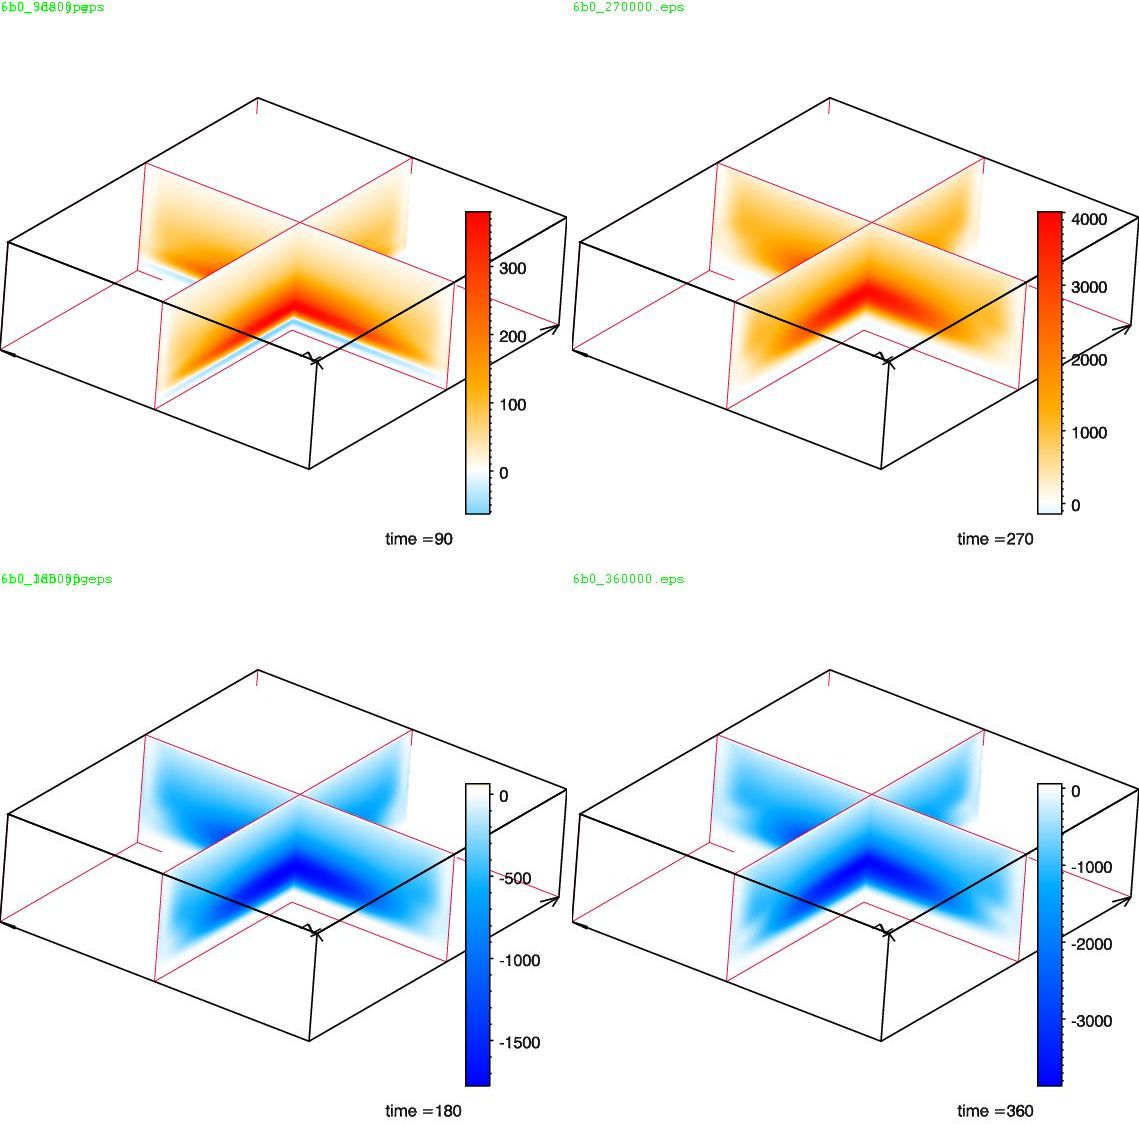
\includegraphics[scale=0.5]{images/6b0_3d.jpg}
\caption{A three dimensional snapshot showing the vertical component of the velocity for the 180s driver for $t=104s$, $t=119s$, $t=134s$ and $t=149s$. }
\end{figure*}
















With the objective of characterising and understanding the nature of the frequencyy shifts of the excited modesWe consider a number of cases

\begin{table*}
\centering
\begin{tabular}{c c c c }
\hline
Label   &  Density Profile & Gravity Enabled & Driver\\
\hline
B &  VALIIC & yes & single driver at photosphere & \\
\hline
C & VALIIC & no & single driver at photosphere &  \\
\hline
D & constant density & yes & single driver at photosphere &  \\
\hline
E & constant density & no & single driver at photosphere &  \\
\hline
F & constant density & no & two drivers at the photosphere and transition zone. &  \\
\hline
\end{tabular} 
\caption{Simulations Used to Characterise Oscillatory Motions Arising from the Surface Driver.}
\end{table*}




%__________________________________________________________________

\section{Magnetohydrodynamic Simulations}



%FIGURE 12 here caption:Magnetic Field Configuration, Alfven Speed, Sound Speed and Temperature Profile for model with constant vertical 10G Magnetic Field$ \\

\begin{figure*}[h]
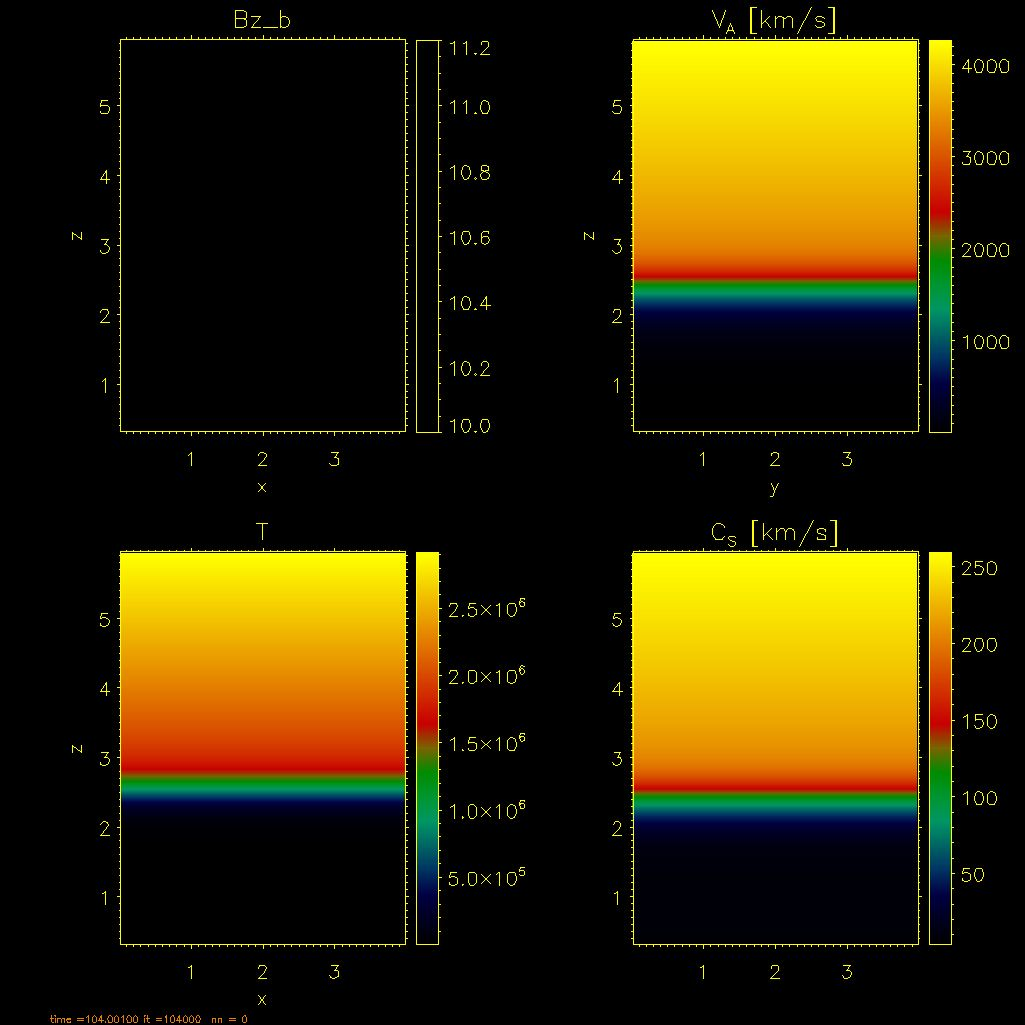
\includegraphics[scale=0.5]{images/s4b0_b1_4field_3d00000.jpg}
\caption{Magnetic Field Configuration, Alfven Speed, Sound Speed and Temperature Profile for model with constant vertical 10G Magnetic Field. }
\end{figure*}



%FIGURE 13 here caption:Magnetic Field Configuration, Alfven Speed, Sound Speed and Temperature Profile for model with 1Mm width Flux Tube \\

\begin{figure*}[h]
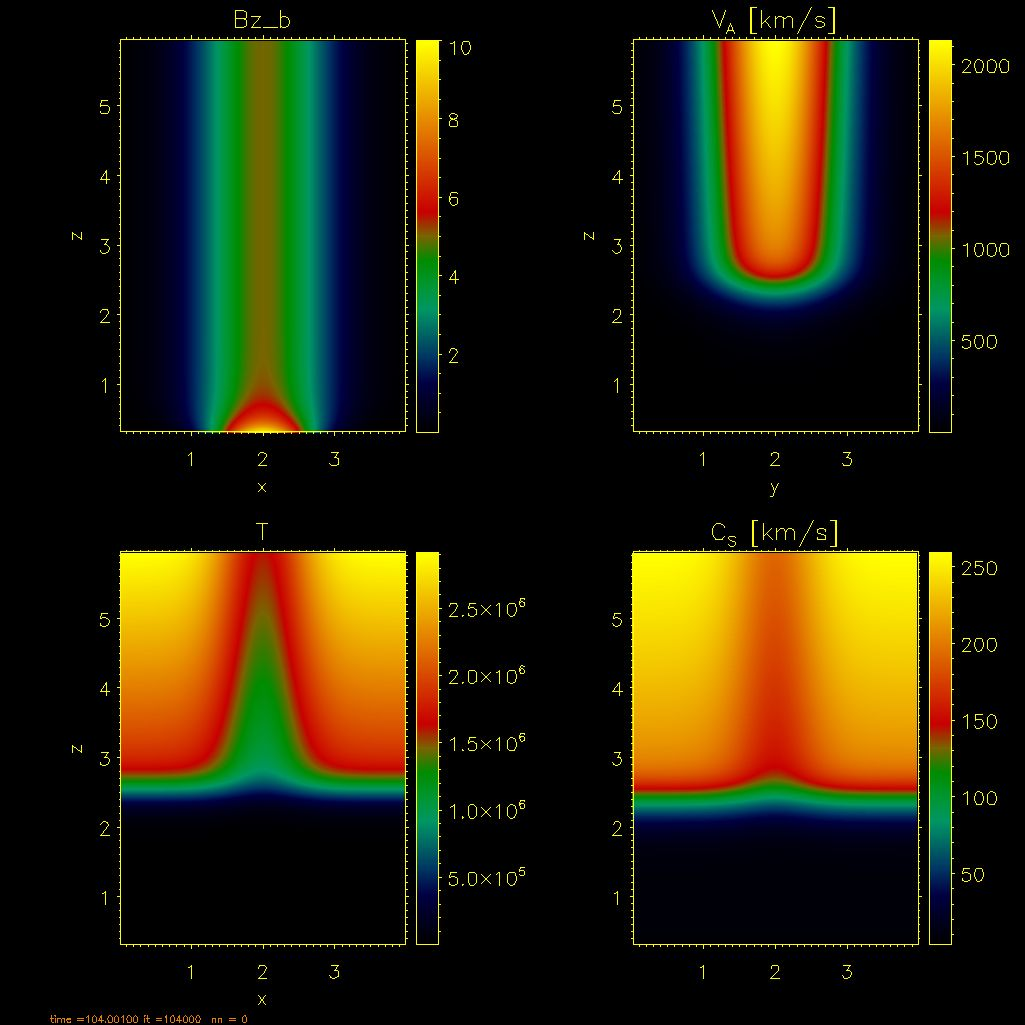
\includegraphics[scale=0.5]{images/s4b0_b2_4field_3d00000.jpg}
\caption{Magnetic Field Configuration, Alfven Speed, Sound Speed and Temperature Profile for model with 1Mm width Flux Tube. }
\end{figure*}


%FIGURE 14 here caption:Magnetic Field Configuration, Alfven Speed, Sound Speed and Temperature Profile for model with 2Mm width Flux Tube \\

\begin{figure*}[h]
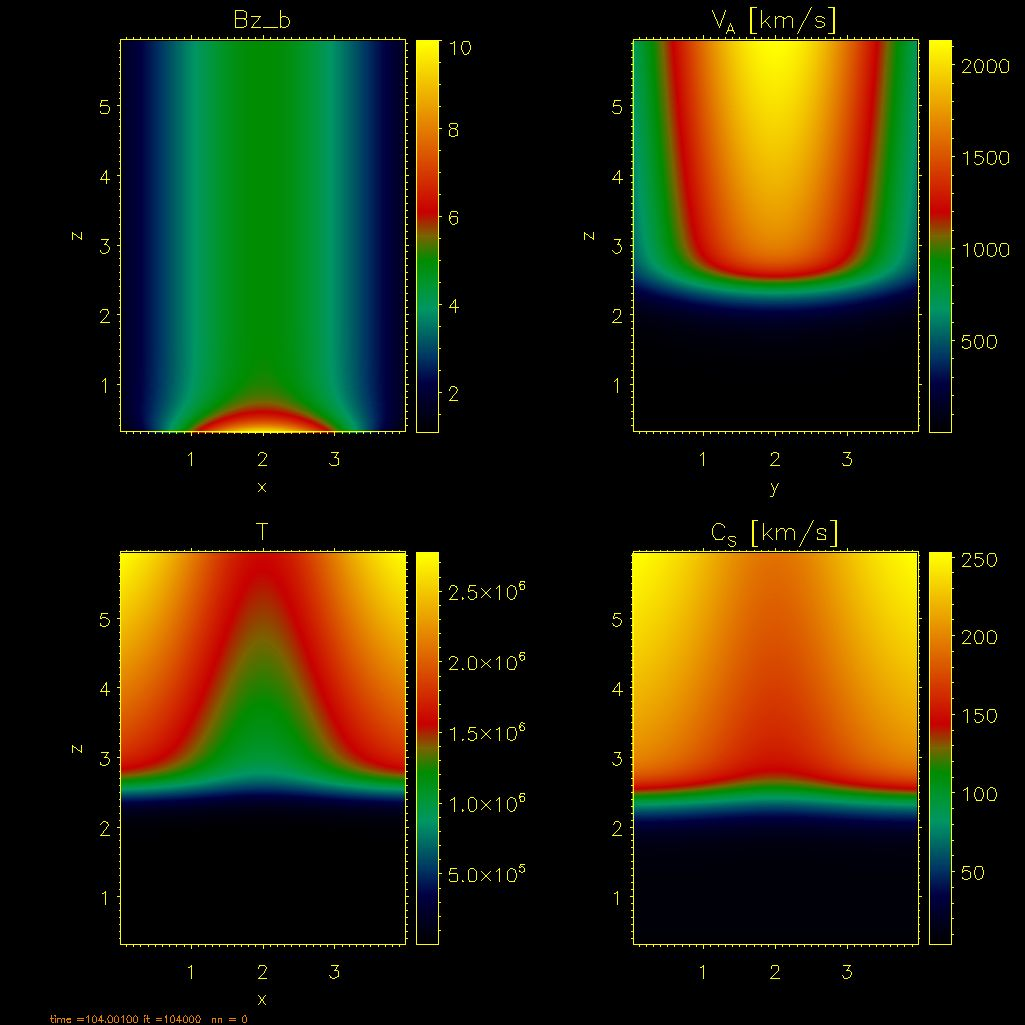
\includegraphics[scale=0.5]{images/s4b0_b4_4field_3d00000.jpg}
\caption{Magnetic Field Configuration, Alfven Speed, Sound Speed and Temperature Profile for model with 2Mm width Flux Tube. }
\end{figure*}



%FIGURE 10 here caption:A three dimensional snapshot showing the vertical component of the velocity for the 30s driver  with uniform vertical 10G Magnetic Field for $t=104s$, $t=119s$, $t=134s$ and $t=149s$ \\

\begin{figure*}[h]
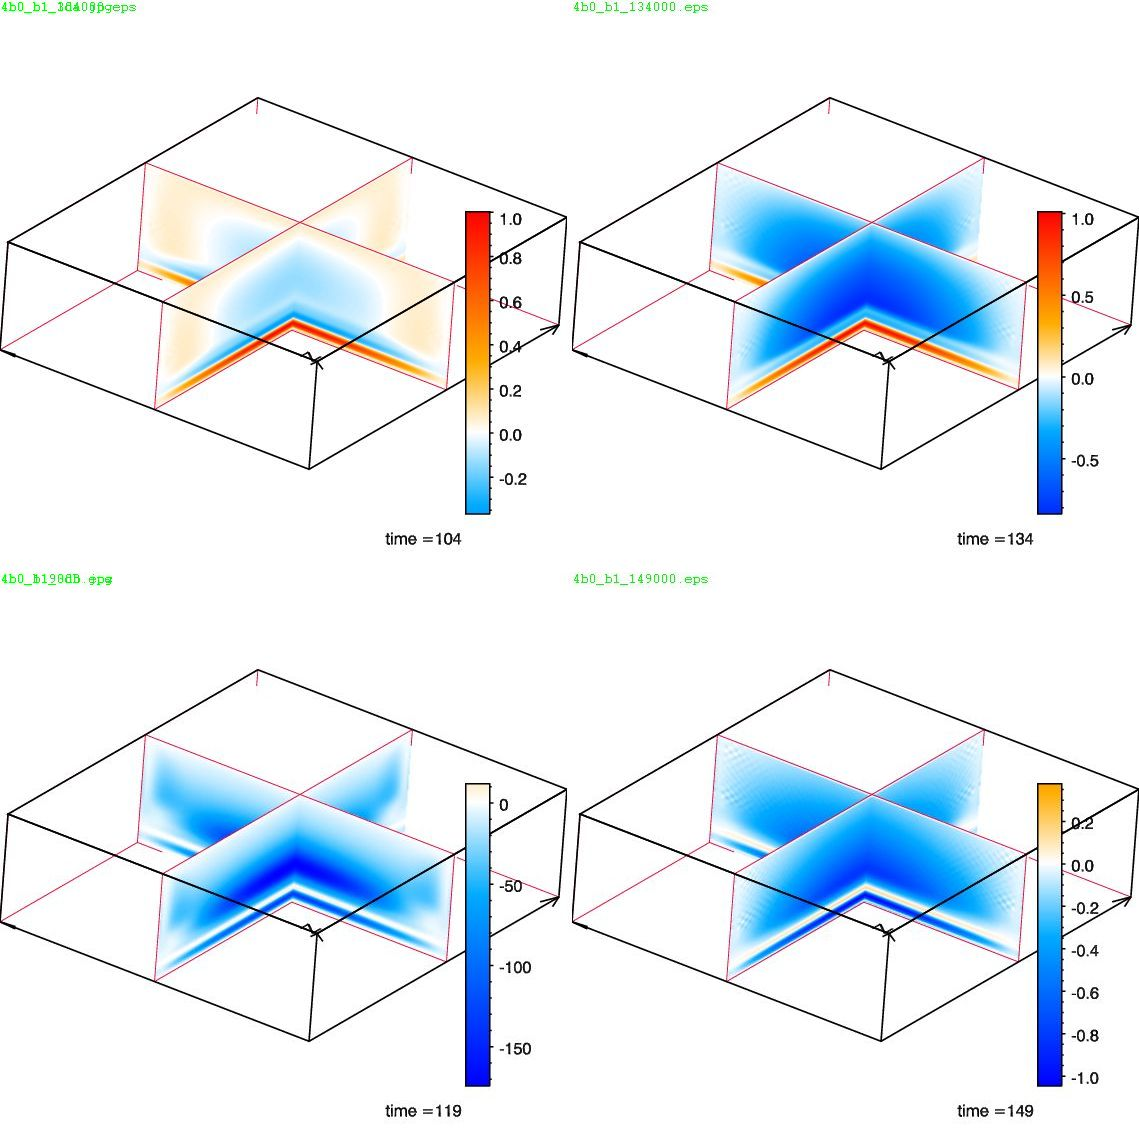
\includegraphics[scale=0.5]{images/4b0_b1_3d.jpg}
\caption{A three dimensional snapshot showing the vertical component of the velocity for the 30s driver  with uniform vertical 10G Magnetic Field for $t=104s$, $t=119s$, $t=134s$ and $t=149s$. }
\end{figure*}



%FIGURE 15 here caption:A three dimensional snapshot showing the vertical component of the velocity for the 30s driver with 1Mm width  10G Magnetic flux tube for $t=104s$, $t=119s$, $t=134s$ and $t=149s. \\

\begin{figure*}[h]
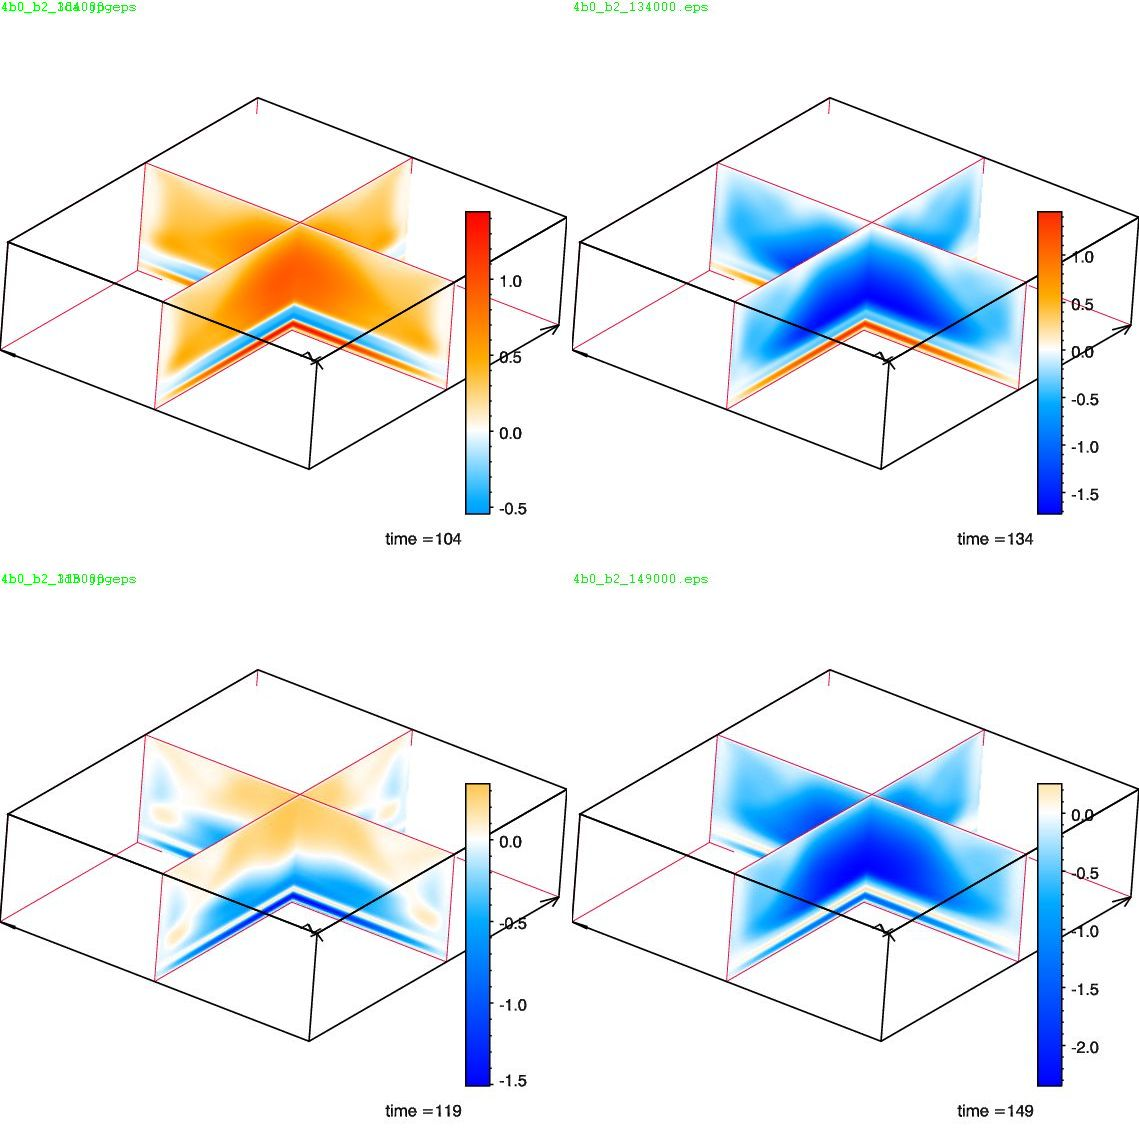
\includegraphics[scale=0.5]{images/4b0_b2_3d.jpg}
\caption{A three dimensional snapshot showing the vertical component of the velocity for the 30s driver with 1Mm width  10G Magnetic flux tube for $t=104s$, $t=119s$, $t=134s$ and $t=149s. }
\end{figure*}





%FIGURE 16 here caption:A three dimensional snapshot showing the vertical component of the velocity for the 30s driver with 1Mm width  10G Magnetic flux tube for $t=104s$, $t=119s$, $t=134s$ and $t=149s. \\

\begin{figure*}[h]
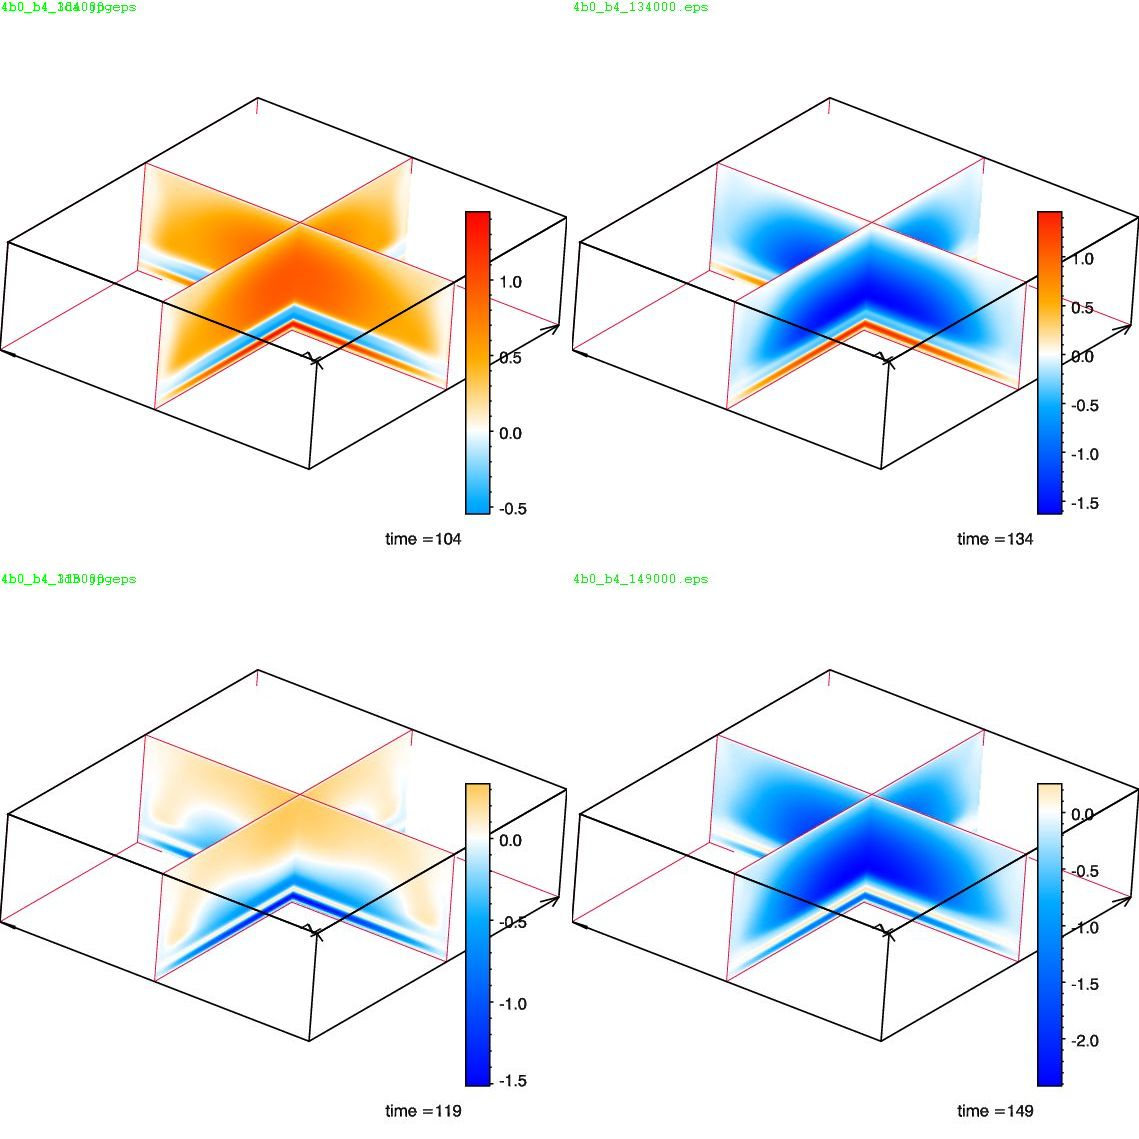
\includegraphics[scale=0.5]{images/4b0_b4_3d.jpg}
\caption{A three dimensional snapshot showing the vertical component of the velocity for the 30s driver with 2Mm width  10G Magnetic flux tube for $t=104s$, $t=119s$, $t=134s$ and $t=149s. }
\end{figure*}
























%______________________________________________________________

\section{Conclusions}

   \begin{enumerate}
      \item The results demonstrate the mode conversion of modes with a 30s period to modes with a 180s period \cite{leibacher1982}. This supports the idea that the chromosphere is a source for the 180s period oscillations.
      \item Increased transition region structuring is observed for the higher order modes
      \item Magnetic flux tube enhance the structruring in the transition zone
   \end{enumerate}

\begin{acknowledgements}
RE acknowledges M. K\'eray for patient encouragement and is also grateful to NSF, Hungary (OTKA, Ref. No. K83133). 
The authors thank the Science and Technology Facilities Council (STFC), UK for the support they received. We acknowledge Corporate Information and Computing Services at The University of Sheffield for the provision of the High Performance Computing Service.
\end{acknowledgements}


%-------------------------------------------------------------------

\begin{thebibliography}{}




\bibitem[Shelyag 2008]{Shelyag2008} Shelyag, S., Fedun, V., \& Erd\'elyi, R. A\&A, 2008, 486, 655

\bibitem[Ulrich 1970]{Ulrich1970} Ulrich, R.K., 1970, ApJ, 162, 993

\bibitem[Leighton 1960]{Leighton1960} Leighton, R.B., 1960,In Thomas R.N. (ed), Aerodynamic Phenomena in Stellar Atmospheres, IAU Symp. 12, 321-325

\bibitem[Fedun 2009]{Fedun2009} Fedun, V. et al,  Solar Phys (2009) 258: 219–241

\bibitem[Srivastava 2013]{Srivastava2013} Srivastava, A.K. et al. 2013 ApJ 765 L42

\bibitem[Leibacher1971]{Leibacher1971} Leibacher, J. W.; Stein, R. F, 1971 ApL 7,191-192

\bibitem[Roth2010]{Roth2010} Roth, M. et al. 2010 ApJ 723 L 175

\bibitem[Marsh2006]{Marsh2006}  Marsh, M. S.; Walsh, R. W. 2006 ApJ 643 540-548

\bibitem[Zhukov 2002]{Zhukov2002} Zhukov, V.I., A\&A, 2002, 386, 653-657

\bibitem[James 2003]{James2003} James, S. P.; Erdélyi, R.; De Pontieu, B., A\&A, 2003, 406, 715-724

\bibitem[Carlsson 1992]{Carlsson1992} Carlsson, Mats; Stein, Robert F., 1992 ApJ 397 L 59

\bibitem[Hindman 1996]{Hindman1996} Hindman, B.W. et al, 1996 ApJ 459 760

\bibitem[Konkol 2012]{Konkol2012} Konkol, P.; Murawski, K.; Zaqarashvili, T. V., A\&A, 2012, 537, 96

\bibitem[Murawski 2010]{Murawski2010}  Murawski, K.; Zaqarashvili, T. V., A\&A, 2010, 519, A8

\bibitem[Cauzzi2008]{Cauzzi 2008}Cauzzi.G. , A\&A, 2008, 480, 515C

\bibitem[Gascoyne2011]{Gascoyne 2011}Gascoyne, A.; Jain, R.; Hindman, B. W. , A\&A, 2008, 526, A93

\bibitem[Jain2011]{Jain 2011}Jain, R.; Gascoyne, A.; Hindman, B. W. , MNRAS, 2011, 415, Issue 2, pp. 1276-1279.

\bibitem[Khomenko2012]{Khomenko2012}Khomenko and Santamaria . 2013JPhCS.440a2048K

\bibitem[Carlsson1995]{Carlsson1995} Carlsson, M.; Stein, R. F., 1995 ApJ 440 L29-L32

\bibitem[Kalkofen2012]{Kalkofen2012} Kalkofen, W., Solar Phys (2012) 276: 75

\bibitem[Leenaarts2011]{Leenaarts2011} Leenaarts, J.; Carlsson, M.; Hansteen, V.; Gudiksen, B. V., A\&A, 2011, 530A, 124L

\bibitem[Vernazza1981]{Vernazza1981} Vernazza, J. E.; Avrett, E. H.; Loeser, R., 1981 ApJS 45 635V

\bibitem[McWhirter1975]{McWhirter1975} McWhirter, R. W. P.; Thonemann, P. C.; Wilson, R., A\&A, 1975, 40, 63-73

\bibitem[Malins2007A]{Malins2007A} Malins, C., Erdelyi, R., Solar Phys (2012) 246: 41-52

\bibitem[Malins2007B]{Malins2007B} Malins, C.,  Astron. Nachr. (2007) 328, No. 8, 752 – 755

\bibitem[Fedun2011]{Fedun2011} Fedun, V. et al, 2011 ApJ 727 17

\bibitem[Leibacher1982]{Leibacher1982}Leibacher,Gouttebroze, and Stein, 1982 ApJ 258 393L

\bibitem[Khomenko2013]{Khomenko2013}Khomenko, E and Irantzu, S, 2013 JPhCS 440a 2048k



\end{thebibliography}

\end{document}

